\documentclass[tikz,border=3pt]{standalone}
\usepackage[T1]{fontenc}
\usepackage[sfdefault]{FiraSans}
\usepackage{newtxsf}
\usepackage{pgfplots}
\usepackage[eulergreek]{sansmath}
\pgfplotsset{compat=1.11}
% % % % % % % % % % % % % % % % % % %DEFINITIONS MINE
\newcommand\mlex{M^{\scriptscriptstyle L}}
\newcommand\msyn{M^{\scriptscriptstyle S}}
\newcommand\mstd{M^{\scriptscriptstyle T}}
\newcommand\slex{S^{\scriptscriptstyle L}}
\newcommand\ssyn{S^{\scriptscriptstyle S}}
\newcommand\sstd{S^{\scriptscriptstyle T}}


\begin{document}
%  \begin{tikzpicture}
%\begin{axis}[
%width=15cm,               %% here, adjust as suitable
%%axis y line=center,
%%axis x line=middle,
%axis lines = middle,  %% instead of above two lines this one is enough
%scaled ticks=false,
%axis equal,
%grid=major,
%xmax=9,xmin=-9,
%ymin=-10,ymax=10,
%xlabel=$x$,ylabel=$y$,
%xtick={-10,...,10},
%ytick={-10,...,10},
%]
%
%\addplot coordinates{(-3,1) (6,-2)};
%\end{axis}
%\end{tikzpicture}

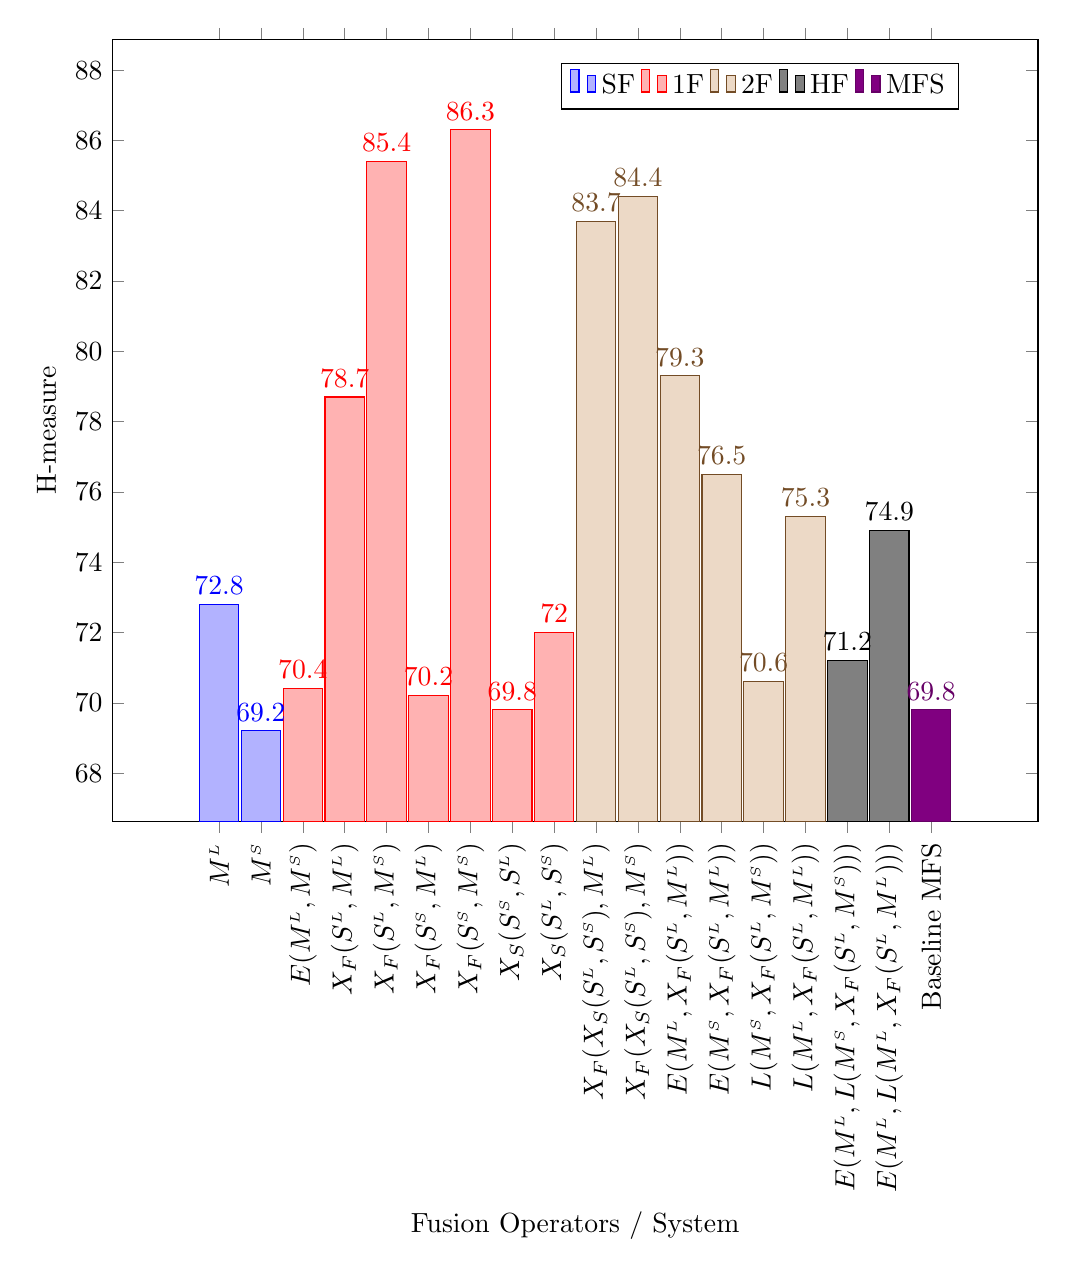
\begin{tikzpicture}
\begin{axis}[
%	xtick distance={160},
    ybar=-0.5cm,
    width=1.1\linewidth,
%    height=\textheight,
    enlargelimits=0.15,
    domain = 0:85,
    xmin=0, xmax=85,
%    x=1mm, % Distance between the centers of the bars
%    enlarge x limits={abs=1cm}, % The distance between the center of the first bar and the left edge
%    enlarge y limits=false,
    legend style={at={(0.7,.97)},anchor=north,legend columns=-1},
    ylabel={H-measure},
    xlabel = {Fusion Operators / System},
    scaled ticks=true,
%    xmin=0, xmax=85,
    xticklabels={
	    {$\mlex$},
	    {$\msyn$},
	    {$E(\mlex, \msyn)$},
	    {$X_F(\slex, \mlex)$},
	    {$X_F(\slex, \msyn)$},
	    {$X_F(\ssyn, \mlex)$},
	    {$X_F(\ssyn, \msyn)$},
	    {$X_S(\ssyn, \slex)$},
	    {$X_S(\slex, \ssyn)$},
	    {$X_F(X_S(\slex, \ssyn), \mlex)$},
	    {$X_F(X_S(\slex, \ssyn), \msyn)$},
	    {$E(\mlex, X_F(\slex, \mlex))$},
	    {$E(\msyn, X_F(\slex, \mlex))$},
	    {$L(\msyn, X_F(\slex, \msyn))$},
	    {$L(\mlex, X_F(\slex, \mlex))$},
	    {$E(\mlex, L(\msyn, X_F(\slex, \msyn)))$},
	    {$E(\mlex, L(\mlex, X_F(\slex, \mlex)))$},
	    {Baseline MFS}
    },
    xtick={0,5,...,85},
    nodes near coords,
    nodes near coords align={vertical},
    x tick label style={rotate=90,anchor=east},
    ]
\addplot+[mark=none, bar width=.5cm]  coordinates {(0,72.8) (5,69.2)};
\addplot+[mark=none, bar width=.5cm]  coordinates {(10,70.4) (15,78.7) (20,85.4) (25,70.2) (30,86.3) (35,69.8) (40,72.0)};
\addplot+[mark=none, bar width=.5cm]  coordinates {(45,83.7) (50,84.4) (55,79.3) (60,76.5) (65,70.6) (70,75.3)};
\addplot+[mark=none, bar width=.5cm]  coordinates {(75,71.2) (80,74.9)};
\addplot+[mark=none, bar width=.5cm]  coordinates {(85,69.8)};

\legend{SF,1F,2F,HF, MFS}
\end{axis}
\end{tikzpicture}

\end{document}